\section{Global Perspectives}
We'll first look into how QIC originated, how different fields like quantum physics, computer science, information theory, cryptography have contributed in it's development. No one would've thought we could process information and do computing using quantum mechanical systems few decades ago.
\subsection{History of QIC}
It all began in the turn of twentieth century, when the "then physics", now known as classical physics resulted in absurdities. Like ultraviolet catastrophe, involving infinite energies and the well known electron spiralling into nucleus in around $10^{-8}$ seconds. Small changes were made everytime, until it resulted in the modern theory of \textit{quantum mechanics} after like a quarter of century. Now it's used in a wide range of fields from structure of DNA to semiconductors to study of nuclear fusion in stars.

\textit{Quantum Mechanics} is a mathematical framework or a set of rules which base our physical theories. For example \textit{quantum electrodynamics} is a fantastic theory built within the framework of quantum mechanics which describes the interaction between atoms and light. It contains it's own set of rules. The rules of quantum mechanics are simple, but even experts found them counter intuitive, one of the main aim of QIC is to build tools which sharpen our intuition of quantum mechanics.

For example, the problem of signalling faster than light, impossible according to Einstein. In quantum mechanics, it converted into the problem whether we \textit{clone} (make a copy of) a quantum state. Even though it is possible in classical mechanics, the \textit{no-cloning} theorem was proved in quantun mechanics. Few imperfect cloning devices were developed which helped us understand it more.

A historical thing which led to the development of QIC is problem of obtaining \textit{complete control over single quantum systems}. The way we used quantum mechanics then had control over a large composite of quantum systems. For example, we could explain superconductivity incredibly well, but we had control over a huge bunch of atoms (quantum systems) to explain that. Slowly, few methods were developed, like isolating an atom by "trapping" it, electron tunnelling microscope which had control over single atoms etc. The reason we tried gaining control over a single quantum system was on a hunch. Most profound insights in science come when we try developing methods to explore new regimes of nature. Famous examples are radio astronomy, low temperature physics etc. In a similar way, there is a hope of discovering new phenomena if we have control over a single quantum system. QIC fits naturally in this problem. A deep understanding and the ability to harness the powers of QIC is essential to gain control over a single quantum system. Despite these efforts, quantum information processing systems have seen modest success, what we can do now is a dozen of operations on few qubits, few real world applications of \textit{quantum cryptography}. It's a challenge now to develop computational methods to take it to a large scale. 

Another big field, a great intellectual triumph, which contributed to QIC is \textit{computer science }. It's history roots back to very old times. But the proper modern incarnation of computer science was announced by \textit{Alan Turing}. \textit{Turing} developed an abstract notion of what we now call as a programmable computer, the \textit{Turing machine}. He also developed the notion of \textit{Universal Turing machine} which could simulate any other turing machine. Another pioneer of computer science, \textit{Alonzo Church}, developed \textit{Church-Turing} thesis, which says if an algorithm can be done on any physical device, an equivalent algorithm is present for a Turing machine, which does the same task. He developed rigorous mathematicalental concepts which are equivalent to what class of algorithms that can be performed by a physical device.

Slowly electrical components like transistors started to develop and programmable computers were made. This growth was codified by \textit{Moore's Law}, which states computer power would double for constant cost roughly every two years. But this law would eventually reach it's limits, as the components would shrink to maximum physical limit. Quantum mechanics would start interfering in the functioning of electrical devices. One possible solution to the failure of Moore's law is to move to a different computing paradigm, which is provided by QIC. A classical computer could simulate a quantum computer, but it's impossible to do it \textit{efficiently}, since quantum computers provided way faster speed. Many reasearchers believe that no \textit{conceivable} amount of development of classical computers would bridge the gap between the powers of a classical computer and powers of a quantum computer.

There are algorithms which are \textit{efficient}, i.e in \textit{computational complexity } terms, they can be solved in polynomial time, others are \textit{inefficient algorithms}. An observation was made which was codified into \textit{strengthened Church-Turing} thesis:-
\begin{center}
    \textit{Any algorithmic process can be simulated effectively using a turing machine.}
\end{center}
But when \textit{analog} computers were developed, theoretically they could solve few problems efficiently which couldn't be efficiently solved by a Turing machine, violating the aforementioned strengthened church-turing thesis. But realistically , considering the noises these couldn't solve the problems efficiently which turing machine couldn't solve efficiently. This consideration of noise was challenge in the development of QIC, which led to theories of \textit{quantum error-correcting codes} and \textit{fault-tolerant quantum computation}. Thus, quantum computers can tolerate a finite amount of noise while having the computational edge.

A major challenge faced by the Church-Turing thesis is when Robert Solovay and Volker Strassen showed that it is possible to find whether an integer is prime or not using a \textit{randomized algorithm}. This could just determine whether a number is \textit{probably} prime or composite with a \textit{certainty}.  At that time, no deterministic primality algorithm was known, neither is now. Hence this suggested that there are efficiently solvable problems which can't be solved efficiently using a deterministic Turing machine. Hence, the strengthened Church-Turing thesis was changed to

\begin{center}
    \textit{Any algorithmic problem can be stimulated efficiently using a \textbf{probabilistic} turing machine.}
\end{center}

This kind of \textit{ad hoc} modification meant that in future there could be some other computational model found which could solve problems efficiently which couldn't be solved efficiently by a Turing machine. Motivated to find a computational model which could simulate any other model of computation, In 1985, David Deutsch tried to look for physical theories which could be a foundation for Church-Turinh thesis which would be as secure as the physical theory, it should simulate any \textit{arbitrary} physical system. Since all laws of physics are ultimately quantum mechanical laws, he considered devices based on principles of quantum mechanics, which were the quantum mechanical analogues of machines defined by Turing, forty-nine years earlier, which now we're considering as a quantum computer.

We still don't surely know whether Deutsch's notion of Universal quantum computer could solve any probleme efficiently. Maybe some mew strange effect from esoteric theories like quantum field theory, string theory, quantum gravity etc. might open a new dimension of computational models, which could solve problems not efficiently solvable by Deutsch's model. Still Deutsch gave a challenge to Church-Turing thesis. Slowly for few problems like finding prime factors of an integer and 'discrete logarithm' problem, it was shown that quantum computing is way superior to classical computing, as it provided an efficient solution while the latter couldn't. It's not possible to simulate quantum mechanical systems on a classical computer, while it is possible on a quantum computer, a problem with profound scientific and technological implications solved.

Coming up with good quantum algorithms which a quantum computer would solve more quickly than a classical computer is difficult. A pessimist might think it's because quantum computers can solve only the problems which have been discovered yet.  But the actual reasons for why designing algorithms for quantum computers are \begin{enumerate*}[label=(\alph*)]
    \item Human intuition is rooted in the classical world, when we use that intuition to construct  algorithms, they'll  be based on classical idea, whic wouldn't use true quantum effects to achieve a good quantum algorithm. Thus we have to turn off our classical intuition while designing quantum algorithms.
    \item  It's not enough to merely design a quantum mechanical algorithm, we have to make it \textit{better} than any exisiting classical algorithm! for which we have to make use of true quantum aspects of quantum mechanics, which isn't a widespread interest because classical algorithms with comparable performace characteristics exist.
\end{enumerate*}
This makes designing quantum algorithms a challenge!

Let's now change our focus to another big contributor to quantum computation and quantum information, information theory. In 1948, Claude Shannon laid the foundation of modern information and communication theory through his papers. The key step taken by Shannon was \textit{to mathematically define the concept of information.} There are \textit{different ways} to define fundamental things like this, which might have their widespread use. But the definition by Shannon is by far the most fruitful in terms of better understanding, a plethora of deep results and a theory with a rich structure which seems to reflect many (not all) real-world communication problems.

Shannon was interested in two key questions which he answered by proving the two fundamental theorems of information theory. Them being
\begin{enumerate*}[label=(\alph*)]
    \item what resources are required to send information reliably over a communication channel? Shannon's first theorem, \textit{noiseless channel coding theorem}, quantifies the physical resources needed to store the output from an information source.
    \item can information be transmitted while being protected against the noises in the communication channel? Shannon's second theorem, \textit{noisy channel coding theorem}, quantifies how much information is possible to reliably sent over through a noisy channel.
\end{enumerate*}
To achieve reliable transmission in presence of noise, Shannon showed that \textit{error-correcting codes} could be used to protect the information. He gave the upper limit of protection it can give, but doesn't give the limiting codes. Many error-correcting codes are being researched and contructed these days, which are reliable enough to be used for computer modems, satellite systems etc. Do not that this is all classical physics.

Quantum information theory followed similar developmenet. First, Ben Schumacher provided an analogue to noiseless channel coding theorem, and defined a 'quantum bit' or 'qubit' as a tangible physical resource. However, no anallogue of noisy channel coding theorem is known till now. However their counterparts have been developed, as theory of quantum error correction, allowing quantum computers to effectively compute in presence of noise, also allowing transfer of data over \textit{noisy quantum} channels effectively. Classical ideas of error-correction have been important in understanding quantum error-correction codes. Slowly, an important class of codes, CSS codes were developed. These were then subsumed \textit{stabilizer codes}, these were felicitated by a deep understanding of classical linear coding theory.

Theory of quantum correcting codes was developed to protect quantum states, against noise, but if we tried to transmit \textit{classical} information, few surprises were found. Like two classical bits of information being transferred by a single qubit, known as \textit{superdense coding}. Another example, \textit{distributed quantum computation}, where we consider two communicating quantum computers, in certain problems, these would take \textit{exponentially lesser time} compared to classical computers connected. But these problems are of little practical application and have technical restrictions, which is a challenge in front of us.

There's also a \textit{networked information theory} which deals with communications with network of many channels. There's not much known about the networked information theory, but the theory is very valuable and gaining insights into it would open up a lot of new things. For example, we have Alice and Bob, they want to send information through a noisy quantum channel which has zero capacity for quantum information. No information is possible to be communicated between them. But suppose we have two such channels operating synchronously, they still have zero capacity. But if we reverse one of the channels, then according to quantum mechanics, this network has non-zero capacity and we can transfer information between them.

\begin{figure}[h]
    \centering
    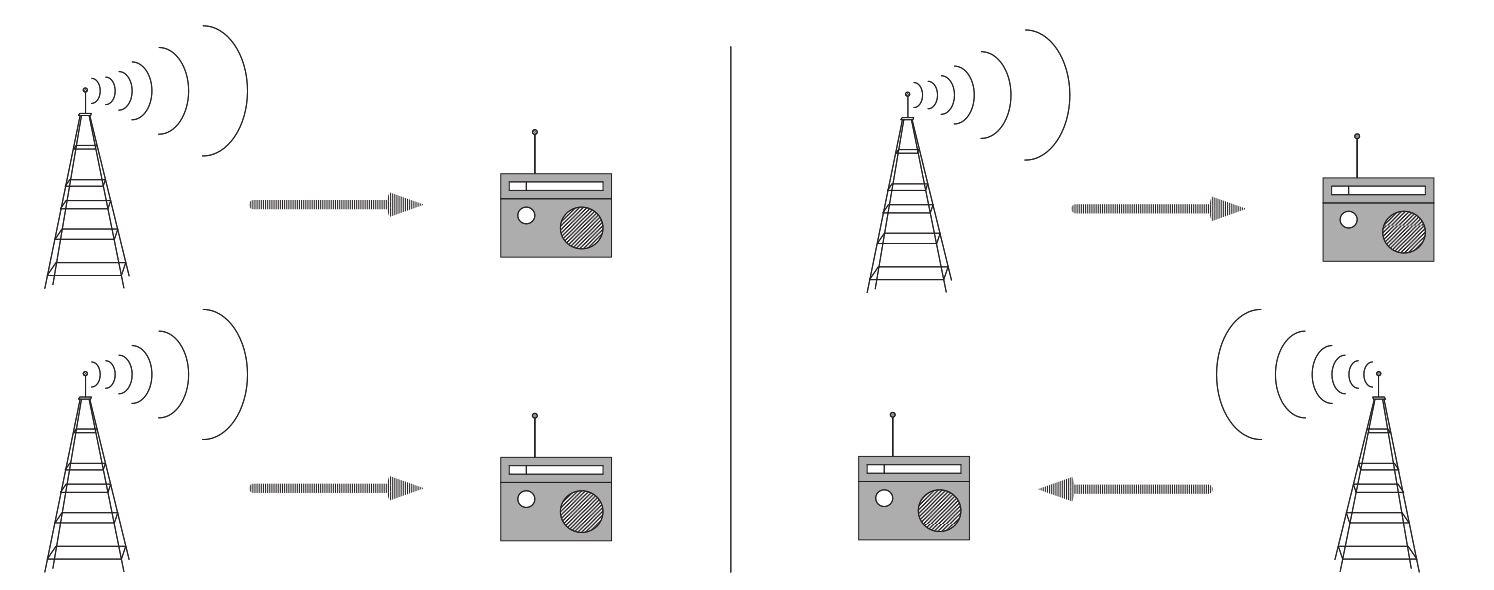
\includegraphics[width=\textwidth]{images/reversing.png} 
    \caption{Reversing one of the channel makes the channel have a non-zero capacity}
    \label{fig:reversing}
\end{figure}

Let's finally move to the respected old art and science of \textit{cryptography}. It's broadly described as the \textit{communication} between two parties \textit{who may not trust each other}. An important case for cryptography is when one party wants to send a secret message to another, without anyone eavesdropping. This is done through a \textit{cryptographic protocol}. Two main ways this can be done is through \begin{enumerate*}
    [label=(\alph*)] \item \textit{public key cryptosystems} \item \textit{private key ecosystems}
\end{enumerate*}.

In \textit{private key cryptosystems}, both party share a private key initially, using which they send \textit{encrypted} messages to each other. Hence only these two can \textit{decrypt} the message, no one else. But the main problem of this is, how are the private keys distributed? what if a third person eavesdrops while they're being distributed? He can get to know every secret message between them. An early discovery of QIC solves this, using \textit{quantum cryptography} or \textit{quantum key distribution}. The basic idea used from quantum mechanics is that if an eavesdropper tries to measure the private key when Alice and Bob are distributing it, they can see that the state of communication channel has changed. Hence they get to know someone's out there and restart it. 

In \textit{public key cryptosystems}, each party makes it's own 'public key', which is made \textit{available to the genreal public}. Using this key of Bob, Alice can encrypt the message. For a third person, it's \textit{extremely difficult} to decrypt this. Not even Alice can decrypt this in real time. Only Bob, who has the keys to his public key personally, can decrypt it. This is most popular these days. The encryption is done through \textit{RSA cryptosystem}. The key here is, it should be extremely decrypt the encryption only with the public key. For this, RSA uses something closely similar to factoring. But Shor's algorithm, run on a quantum computer can to this effectively. Few use discrete logarithm problem, which can also be done effectively by Shor's algorithm. This implies a need of quantum computing and quantum information.

The most striking of these in the study of \textit{quantum entanglement}. It is a unique quantum mechanical \textit{resource} which plays a key role in many applications of QIC. It's like iron to the classical world's bronze age. There's no proper theory of quantum entanglement as of now, a lot of effort is being made. Further study of quantum entanglement is going to lead to amazing new discoveries in quantum computation and quantum information.

\subsection{Future Directions}
As we've looked into the brief history of quantum computation and quantum information, it has something to offer to science, technology and humanity. Quantum computing and quantum information has taught us to \textit{think physically}, yielding new capabilities for information processing and computation. Even computer scientists and information theorists have got a new paradigm to explore upon. We've also learnt that \textit{any physical theory} can be used for information processing and computation. These might one day result in information processing devices with capabilities way beyond current systems. 

Quantum computing and quantum information also offers few important things to physicists. It makes us think physically about computation, but learning to \textit{think computationally about physics} would lead to new things. Traditional physics deals with 'elementary' particles, it's fine but there are many interesting phenomena discovered when larger and complicated things are considered. Chemistry, engineering do it, but it's in an \textit{ad hoc} way. Quantum computing and quantum information provides a way to study such systems. Quantum algorithms and computations allow us to simulate and understand complex physical systems, giving new insights. One day, we might have a good understanding of all aspects of physics.
